\section{State of the Art} \label{sec:sota}
This section will discuss the existing smart materials that are currently studied and used in the domain of actuators. The different techniques and integration systems will also be presented with the goal to compare the various approaches currently used.

\subsection{Smart materials} \label{subsec:Smartmaterials}
In the field of engineering, ranging from haptics, automation and bio-medical fields, there has been a need  to create actuators that are lightweight, compact and having force output. This creates a need for materials that can deliver high forces and strokes while remaining light and small meaning that the materials need to have a high work output.

On the basis of creating an actuator that can meet the demands of the currently implemented strategies while at the same time pushing the limits of the current technology, a thorough investigation of the available smart materials must be conducted. These materials have the ability to react to an external stimulus such as thermal electrical or magnetic and are thus referred to as \emph{smart} or \emph{active materials}. These materials have an inherent property that allows them to be exploited with a specific external stimulus so as to alter their mechanical characteristics or to create self-sensing technology.

There exist numerous types of smart materials and based on their properties, they can be classified into many types such as \cite{damodharan_review_2018}:
\begin{itemize}
	\item Piezoelectric materials
	\item Magneto-strictive materials
	\item Electro-active polymers
	\item Shape Memory Alloys
\end{itemize}

The aim of this project is to adapt these aforementioned smart materials to harness their specific behaviour and fabricate smart actuators. This implies that the system that incorporates the material is equally critical for the conception of the actuator. This section of the report will delved into different strategies used to harness the specific behaviours of the smart materials and integrate them into actuators.

\subsubsection{Piezoelectric Materials}
Piezoelectric materials are a subgroup of smart materials that have the capability to produce voltages when a stress is applied. This behaviour is can also be expressed in the opposite direction i.e. a strain can be generated using an electric field. Piezoelectric materials are the most popular type of smart materials and the most commonly used piezoceramics, such as lead zirconate titanate, are available in the form of thin sheets. These sheets can then be stacked to create piezostack actuators.

\subsubsection{Electro-Active polymers}
Electroactive Polymers (EAP) are smart material polymers that have the ability to alter their mechanical behaviour such as a change in shape or size when exposed to an electric field. They are most commonly used in the domain of actuators and sensors. EAPs emerged in the last few decades exhibiting large strains when exposed to electrical stimulus \cite{bar-cohen_artificial_2005}.

EAP can generate high strains, with Dielectric elastomers (DE) such as silicone exhibiting strains of about 63\%\cite{kornbluh_electroactive_2004}. Generally, these materials can generate strains much greater than rigid and fragile piezoeletric ceramics. EAP materials can also exhibit greater response times when compared to smart materials such as shape memory alloys, which will be explored in the next section. EAP can be very useful for their fast actuation times, low density and greater resilience and can, thus, be very convenient when create mechanical devices that are light weight and compact.

Dielectric Electroactive Polymers (DEAP) are based on the electromechanical behaviour of dielectric films when a compliant electrode is placed on each surface and a voltage is applied across them. This results in the DEAP to shrink in thickness and expand in area.

\begin{figure}[H]
    \centering
    \begin{subfigure}[t]{0.45\textwidth}
			\includegraphics[width=\textwidth]{Figures/DEAP_fig.png}
			\caption{Functional element of dielectric elastomer actuators. Polymer film compresses in thickness and expands in area when a voltage is applied across the film.}
			\label{fig:DEAP_fig}
    \end{subfigure}
    ~ %add desired spacing between images, e. g. ~, \quad, \qquad, \hfill etc.
      %(or a blank line to force the subfigure onto a new line)
    \begin{subfigure}[t]{0.45\textwidth}
			\includegraphics[width=\textwidth]{Figures/DEAP_curve.png}
			\caption{Typical thickness or planar strain response to applied electric field for a film with no external loads.}
			\label{fig:DEAP_curve}
    \end{subfigure}
		\caption{Principle of operation of dielectric elastomer actuators\cite{kornbluh_electroelastomers:_2002}.}
		\label{fig:DEAP}
\end{figure}

The behaviour of the film is caused by the interaction of the electrostatic charges that are created on the opposing electrodes. By applying a voltage on the two electrodes, the electrodes are subjected to opposite charges cause an attractive force between them. The pressure, $p$, created can be calculated\cite{thummala_analysis_2012} using the following relationship :
\begin{equation}
	\label{eq:DEAP_p}
	p = \varepsilon_r\varepsilon_0E^2 = \varepsilon_r\varepsilon_0(V/t)^2
\end{equation}
where $\varepsilon_r$ and $\varepsilon_0$ are the permittivity of free space and the relative permittivity of the polymer respectively, $E$ is the electric field, $V$ is the voltage applied across the electrodes and t is the thickness of the dielectric material.

\begin{wrapfigure}{r}{0.4\textwidth}
	\centering
	\vspace{-20pt}
	
\includegraphics[width=0.35\textwidth]{Figures/IPMC_fig.png}
	\caption{IPMC actuation principle\cite{poubel_proposal_2011}.}
	\vspace{-15pt}
	\label{fig:IPMC_act}
\end{wrapfigure}

Another variant of the EAPs are the Ionic EAP which differ from the DEAP which are sometimes referred to as Electronic EAP\cite{bar-cohen_artificial_2005}. The difference between the two variants arises from the fact that the actuation in Ionic EAPs is a result of diffusion of ions while in the traditional EAP, it is driven by Maxwell forces. An interesting Ionic EAP material are Ionic polymer-metal composites (IPMC). These IPMCs are a type of synthetic composite material that has a muscle-like behaviour under an applied voltage or electric field. In figure \ref{fig:IPMC_act}, the working principle is shown where as a voltage is applied, the diffusion of ions within the material causes a deformation. They are generally ionic polymers that are chemically plated with conductors\cite{shahinpoor_ionic_1998}.

IPMC bending actuators have been used primarily used as bending actuators and artificial muscles. A novel work conducted by J. Rossiter in 2006\cite{rossiter_self-switching_2006} where a self-switching strategy is explored within the scope of a buckled bistable beam made entirely of the IPMC smart material. The work addresses many disadvantages experienced by using a classical bistable buckled beam system with an external trigger mechanism such as relaxation after actuation. low repeatability and the need for energy to maintain the stable states. The work concludes that by use of self-switching system, where the material itself is used as the buckled monolithic beam and switches from one stable state to another using applied voltage, the aforementioned disadvantages can be addressed. In this work, a buckled monolithic IPMC beam is separated into a number of electrically independent segments. The work, then, proposes various strategies to activate the segments so as to actuate the beam into transitioning or bifurcating from one of the stable positions to another.
\begin{figure}[!htb]
	\centering
	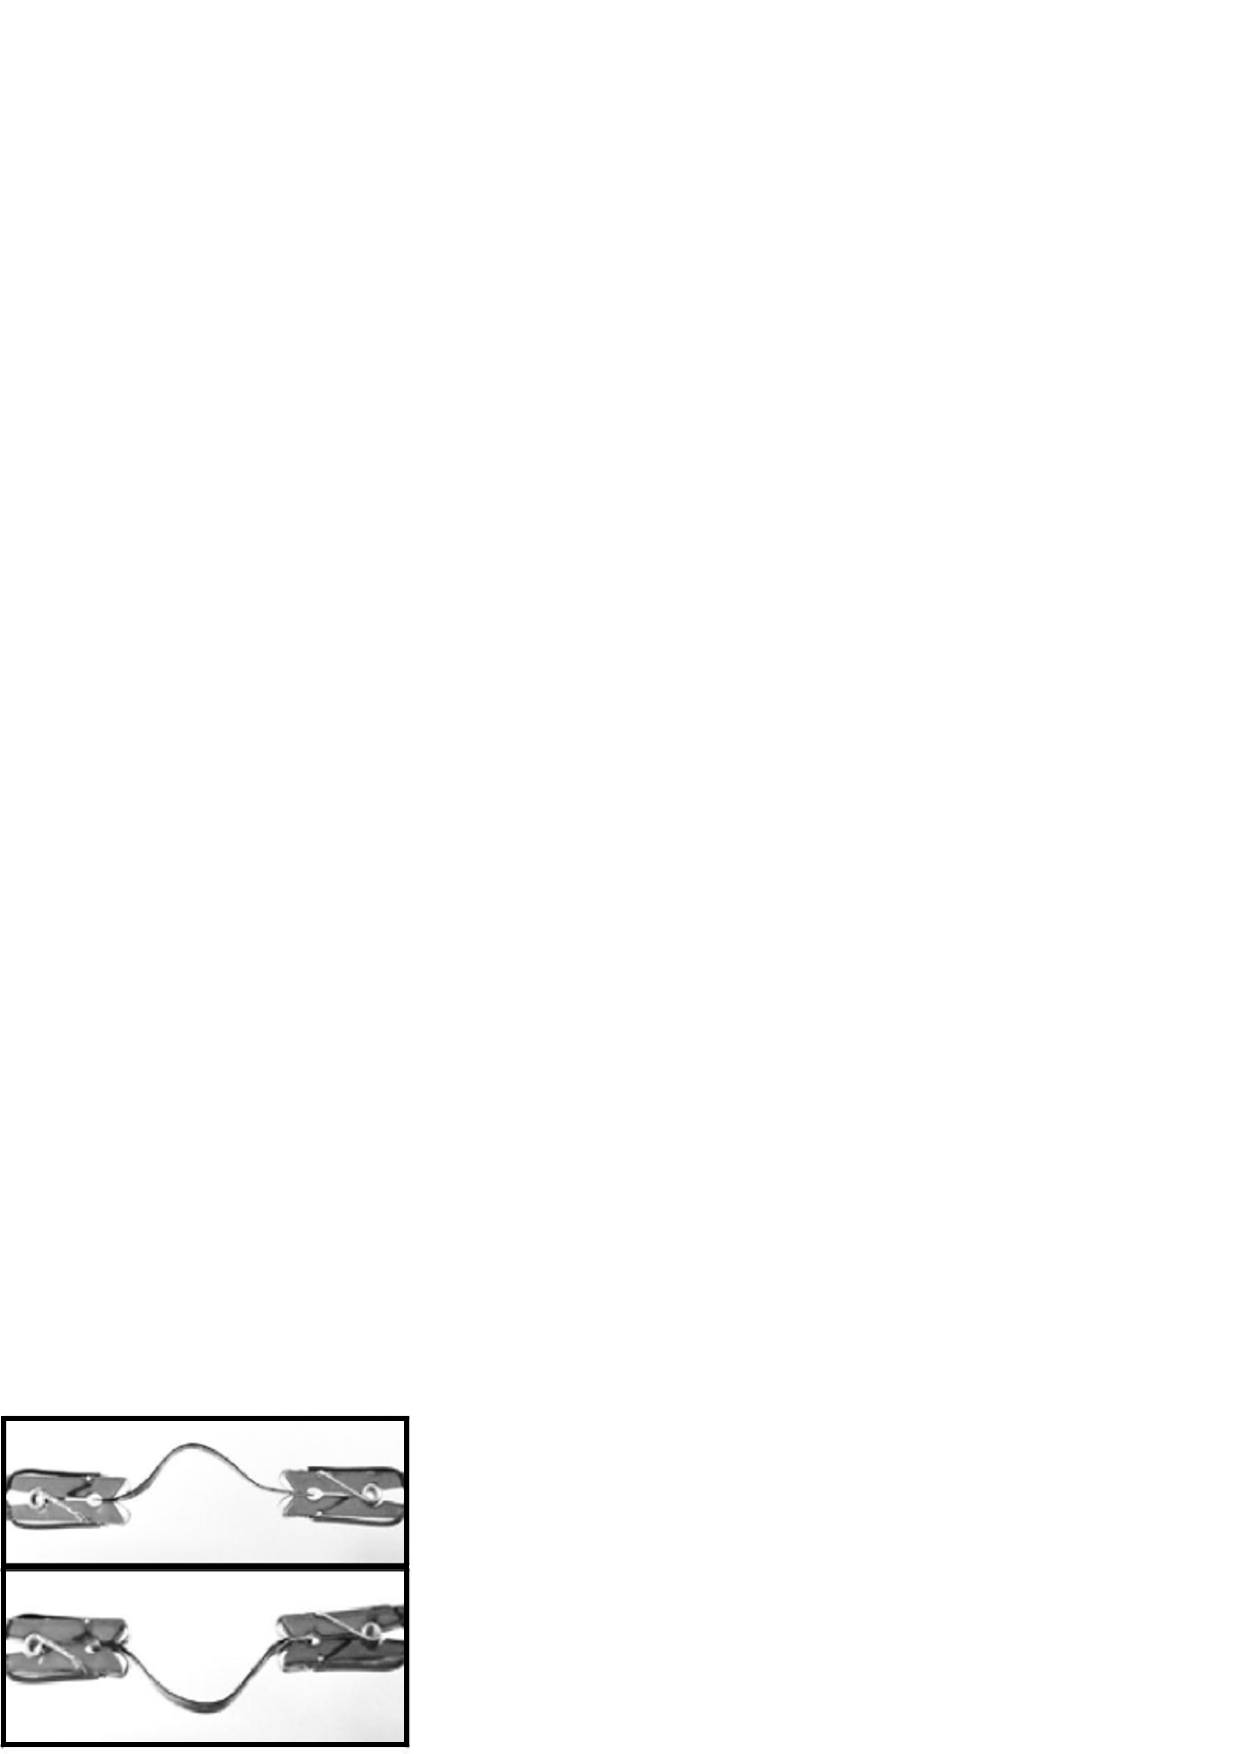
\includegraphics[width=0.95\textwidth]{Figures/IPMC_buckle.png}
	\caption{}
	\label{}
\end{figure}
\begin{figure}[!htb]
	\centering
	\includegraphics[width=0.95\textwidth]{Figures/IPMC_segment.png}
	\caption{}
	\label{}
\end{figure}
\subsubsection{Magneto-strictive materials}
The magneto-strictive materials are category of smart materials that have the ability to alter their mechanical behaviour and shape when subjected to magnetic fields. Magnetic Shape Memory Alloys (MSMA) are a popular type of magnet0-strictive material. Here, the MSMA shows an interesting behaviour in which the material when deformed will tend to remain stable and retain its deformed shape. As the materials is introduced into a strong magnetic field, the crystals of the material are realigned and the material reverts back to its predeformed shape.

\subsubsection{Shape Memory Alloys}
Shape Memory Alloys (SMA) are a particular subgroup of smart materials that change their mechanical behaviour based on a thermal stimulus. Here, the material as with the MSMA, retains its shape when deformed and reverts back to its original shape when heated. Shape Memory Alloys (SMA) actuators provide us with an opportunity to create such actuators due to their high work output per volume which is around 10 $\mathrm{J}/\mathrm{cm}^3$\cite{mohd_jani_review_2014}. This can be a 10-fold increase when compared to pneumatic actuators. The SMA actuators are thus able to provide large amounts of force when compared to their volume, making them particularly useful in compact, lightweight actuators.

NiTiNOL, the most used SMA, contains an interesting property known as the Shape Memory Effect (SME), which allows the material to return to its unloaded state when it is heated above its transition temperature.

Shape memory alloys such NiTiNOL show two important properties: the Shape Memory Effect (SME) and Superelasticity (SE)\cite{rao_design_2015}. The property, this device aims to exploit is the SME. Materials exhibitng this property are able to return to a pre-defined shape when heated through a certain temperature range.

SMAs exist in various different stable phases which consists of the \emph{Martensitic (M)} phase and the \emph{Austenitic (A)} phase. The M phase can exist in either the \emph{Twinned M phase} or the \emph{Detwinned M phase} based on the stress experienced by the material. The SME is the effect that transforms the material from the A phase to its M phase, also known as the Martensitic transformation. The opposite transformation, from the M phase to the A phase, is known as Austenitic transformation. When the material reaches the Austentic transformation temperature ($\mathbf{A_s}$) threshold, the material will begin the Austenitic transformation. Inversely, as the material cools down to the Martensitic transformation temperature ($\mathbf{M_s}$), it will begin the Martensitic transformation. Since these transformations occur over a range in temperature, we must heat and cool well beyond the transformation temperatures.

\begin{wrapfigure}{r}{0.5\textwidth}
  \centering
  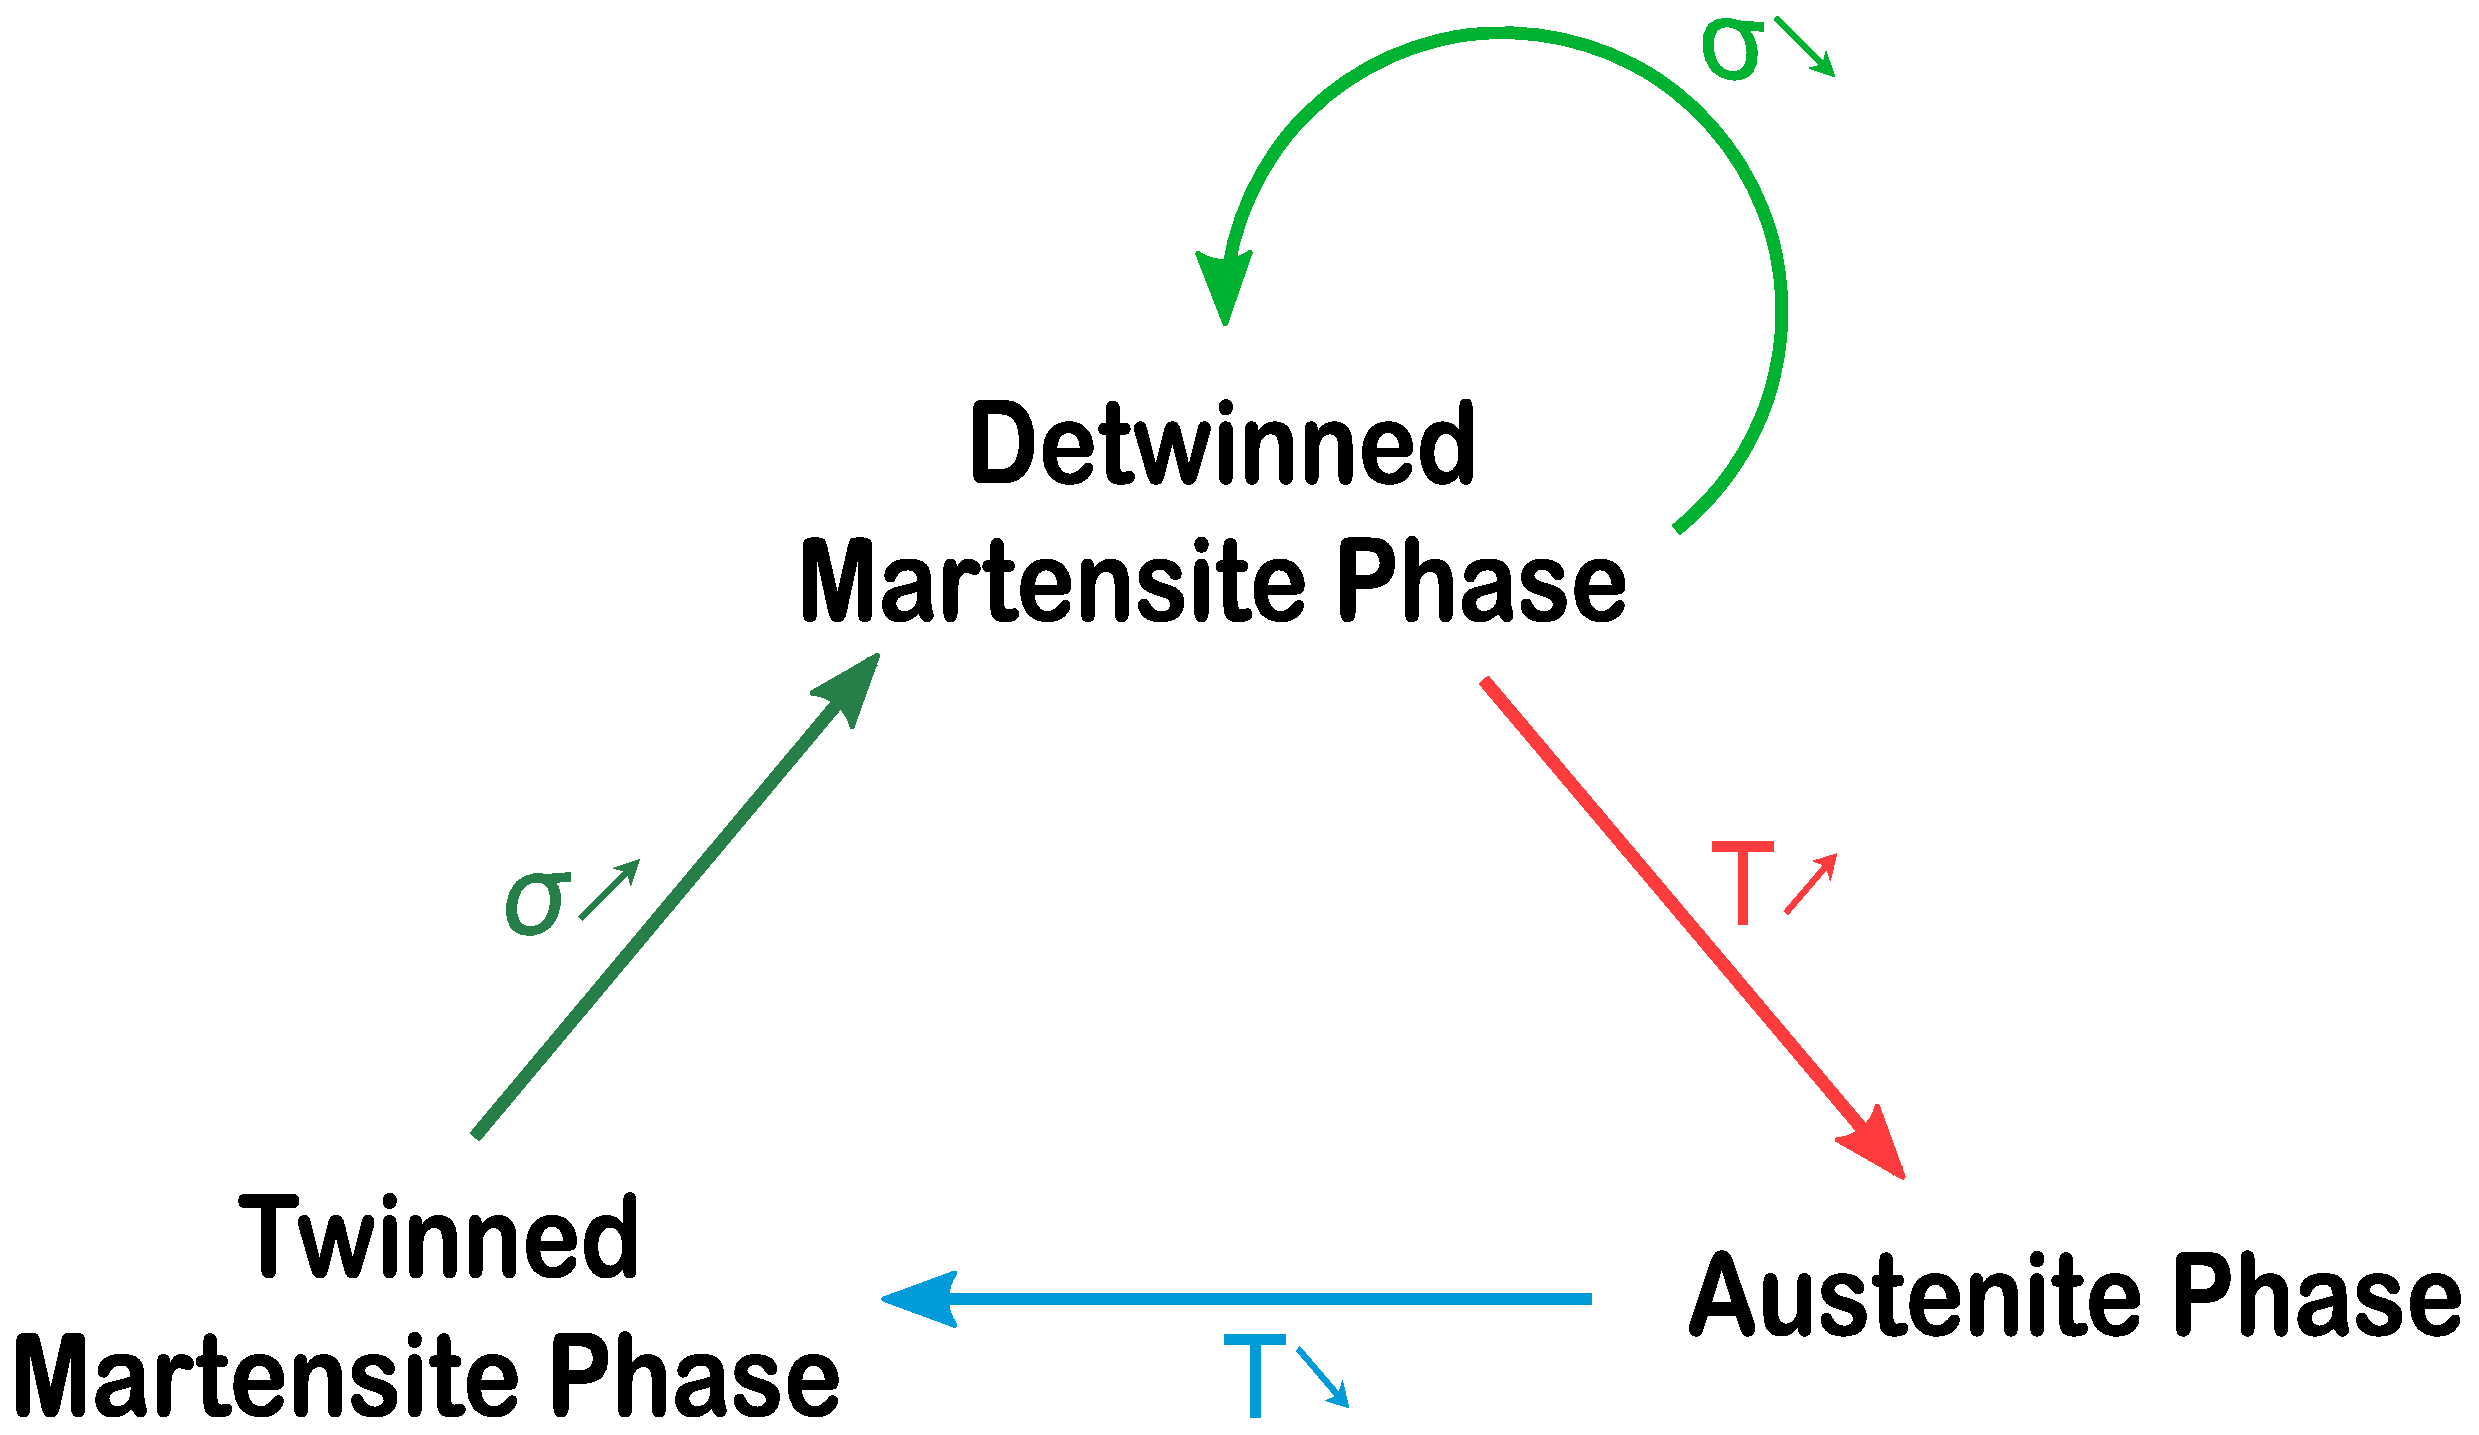
\includegraphics[width=0.48\textwidth]{Figures/Phase_Transf_Diagram_noText.eps}
  \caption{Phase transformation diagram of a shape memory alloy. Here $\sigma$ represents the stress created by mechanical loading and T represents the temperature change due to thermal loading.}
	\vspace{-10pt}
  \label{fig:PhaseTransfDiagram}
\end{wrapfigure}


The SMA that in most likelihood will be used is a type of NiTiNOL variant with a relatively high transformation temperature (with $A_s$ around 50\degreeC) and thus exists primarily in the M phase at room temperature. The phase transformations can be seen in figure \ref{fig:PhaseTransfDiagram}. When a mechanical load is applied to the SMA while in its M phase, the material shears on an atomic level and this allows it to deform through a detwinning process at relatively low stress levels. This process allows the material to deform up to strains of 8$\%$. Strains larger than this will cause dislocations which are irreversible. When the beam is then heated, the Austentite transformation from the detwinned M phase to the A phase, causes the beam to lose all the strain due to twinning, allowing the material to return to its original shape. This strain recovery allows the beam to revert to its pre-defined state while producing large forces.
